\section{典型效应}
这一节中我们用 $ l $ 来表示线长.
\subsection{钟慢效应}
考虑两个在惯性系 $ \mathcal{R} $ 中静止的标准钟 $ C_1 $, $ C_2 $ 和一个在惯性系 $ \mathcal{R}' $ 中的静止的标准钟 $ C' $, 它们的世界线如图 \ref{time dilation} 所示.

\begin{figure}[htbp]
    \centering
    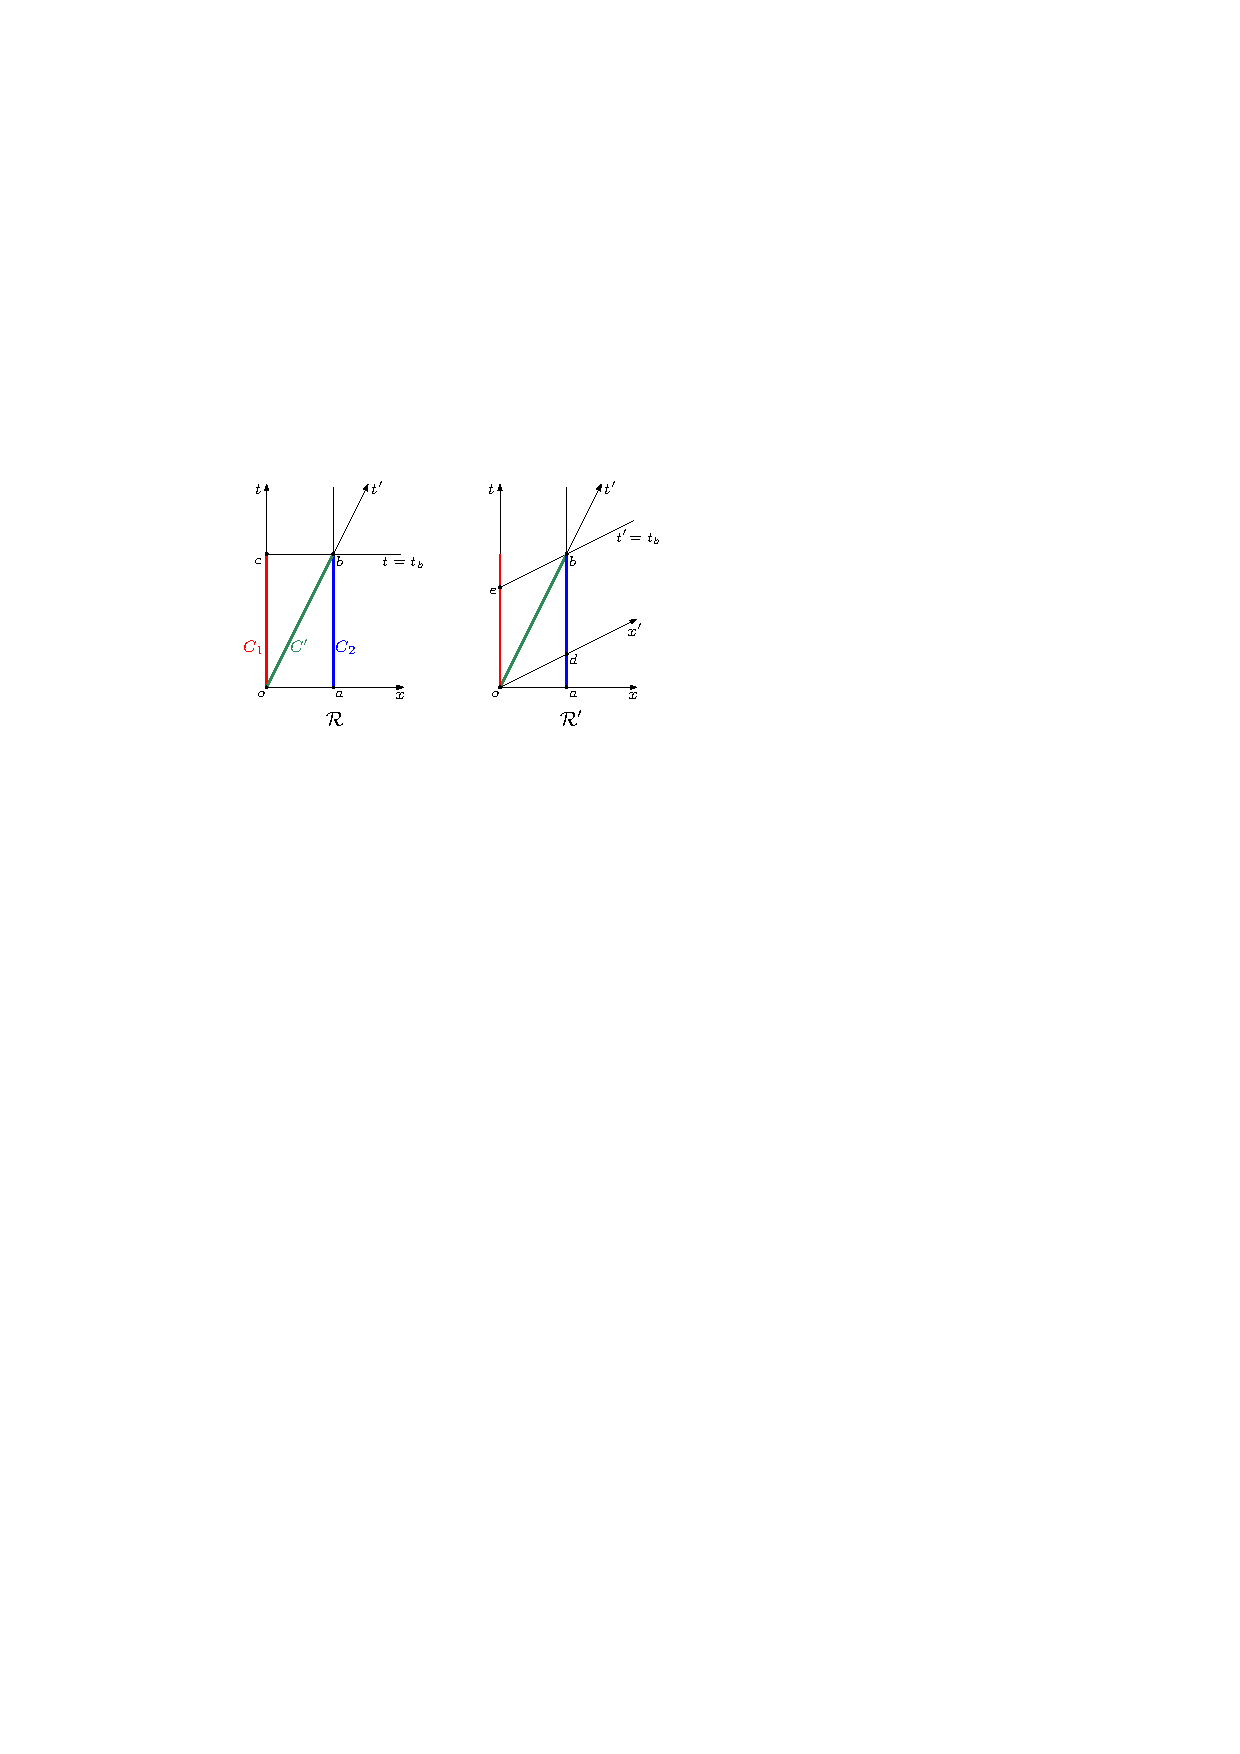
\includegraphics[width=0.8\textwidth]{pic/time dilation.pdf}
    \caption{time dilation}
    \label{time dilation}
\end{figure}

先在 $ \mathcal{R} $ 系的视角中进行讨论, 当 $ t=0 $ 时我们将三个钟的读数都调为 $ 0 $, 此时 $ C' $ 与 $ C_1 $ 重合; 当 $ t=t_b $ 时, $ C' $ 与 $ C_2 $ 重合, 此时 $ C_2 $ 的读数为 $ l_{ab}=t_b$, $ C' $ 的读数为 $ l_{ob}=\sqrt{t_b^2-x_b^2}<l_{ab}$, 因此在 $ \mathcal{R} $ 系看来钟 $ C' $ 走慢了.

\begin{remark}
    上述讨论中有一些细节需要注意:
    \begin{enumerate}
        \item 在一个参考系中, 我们称所有时间分量相同的点所构成的集合为同时面, 语句 ``当 $ t=0 $ 时'' 应理解为语句 ``在 $ t=0 $ 的同时面上'' 的缩写.
        \item 只有在两个钟重合于某一点时才能比较读数, 比如当 $ t=t_b $ 时, $ C' $ 只能和 $ C_2 $ 比较读数, 不能和 $ C_1 $ 比较读数.
        \item 信息的传播需要时间, 若 $ C_1 $ 将自己读数调为 $ 0 $ 的同时告诉 $ C_2 $ 调读数, 那 $ C_2 $ 收到消息并将读数调为 $ 0 $ 时, $ C_1 $ 的读数已经不是 $ 0 $ 了. 钟 $ C_1 $ 和 $ C_2 $ 在 $ t=0 $ 时读数都为 $ 0 $ 这个条件叫做{\bf 钟同步} (clock synchronization), 一个实现钟同步的方法如图 \ref{clock synchronization} 所示: $ C_1 $ 朝 $ C_2 $ 发射一束光并记下自己的读数 $ t_1 $, $ C_2 $ 手持一面镜子将光反射回去, $ C_1 $ 在收到反射回来的光时记下自己的读数 $ t_2 $ 并计算读数差 $ \Delta t=t_1-t_2 $, 接下来 $ C_1 $ 再发射一束光并在自己的读数增加 $ \Delta t/2$ 后将自己的读数调为 $ 0 $, 而 $ C_2 $ 再次接收到光时也将自己的读数调为 $ 0 $. (这一方法利用了光速与方向无关的假设)
    \end{enumerate}
    \begin{figure}[htbp]
        \centering
        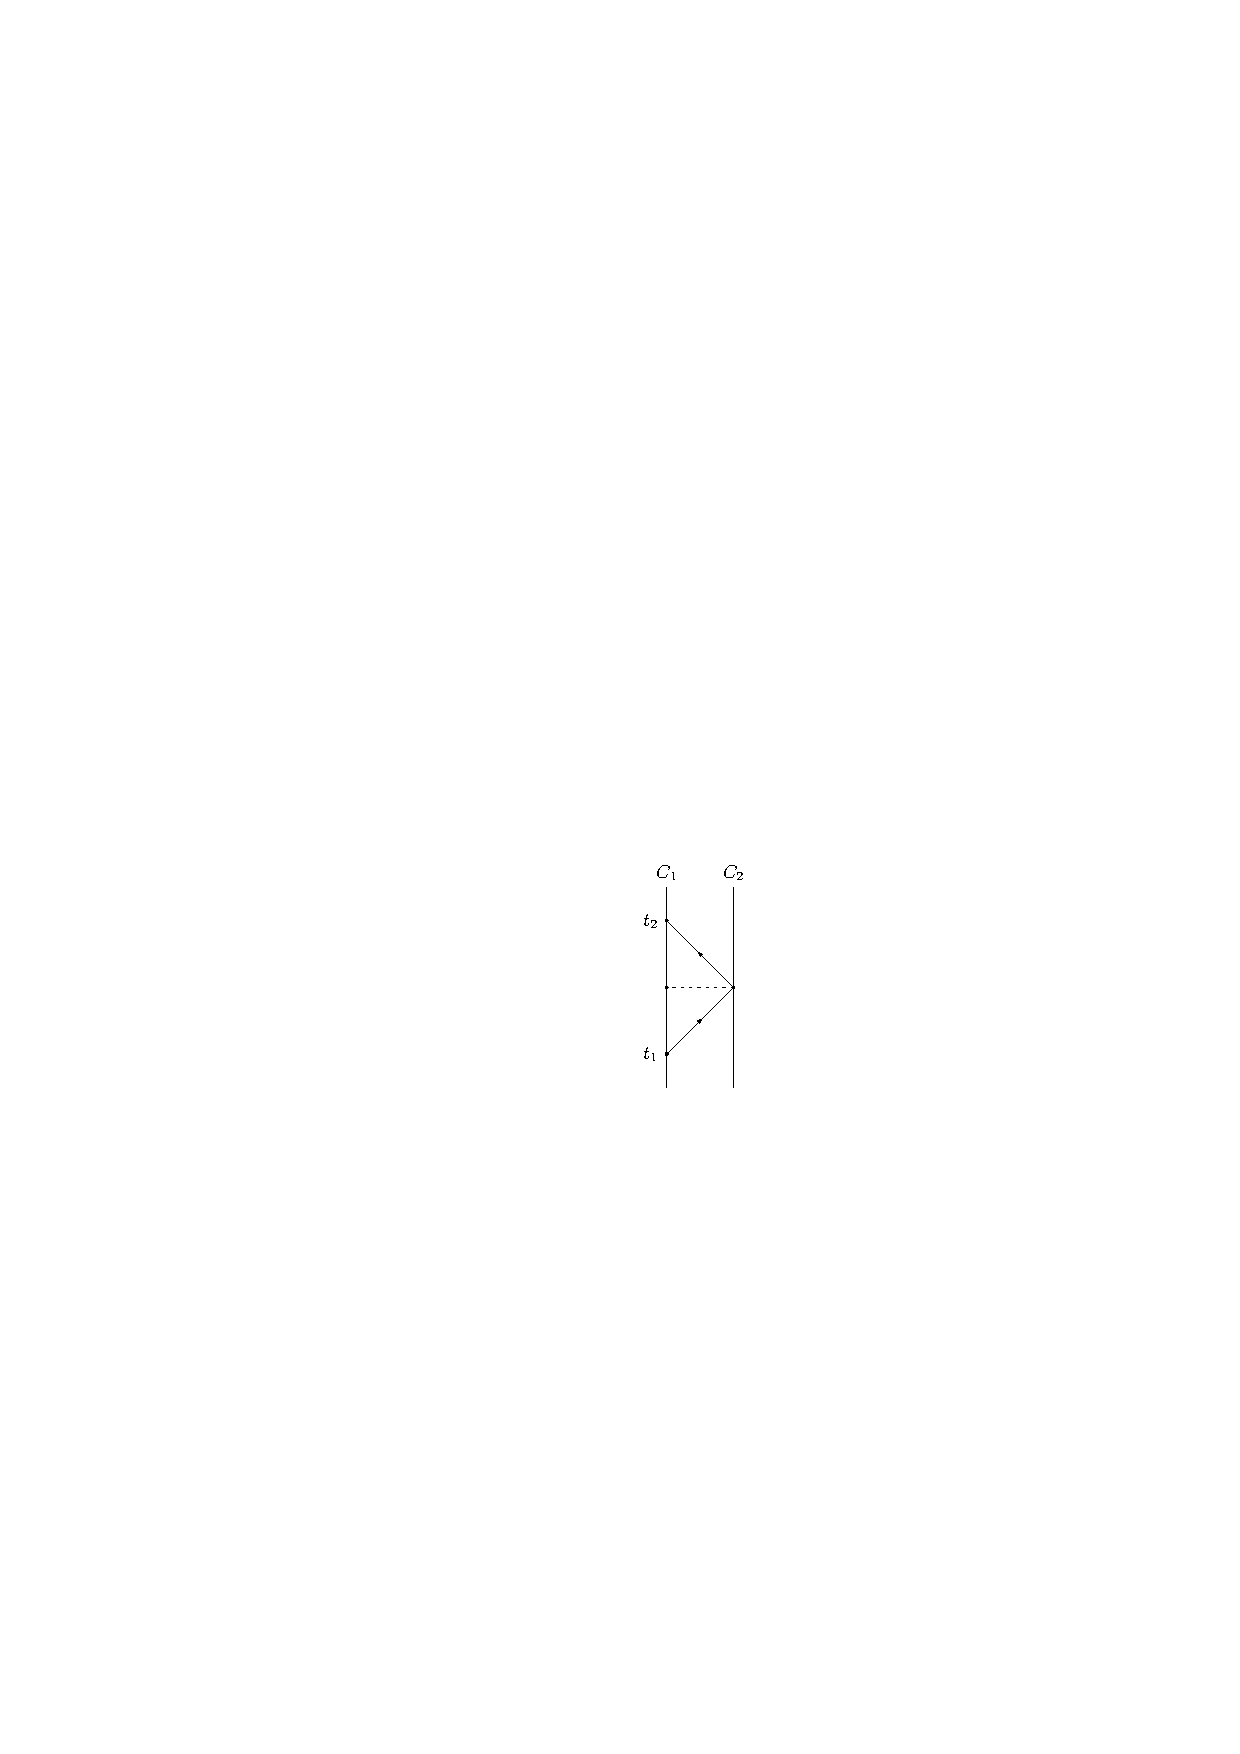
\includegraphics[width=0.2\textwidth]{pic/clock synchronization.pdf}
        \caption{clock synchronization}
        \label{clock synchronization}
    \end{figure}
\end{remark}

在 $ \mathcal{R}' $ 系的视角中, 事件 $ o $ 与 $ d $ 是同时的, 此时 $ C_1 $ 和 $ C' $ 的读数为 $ 0 $, 而 $ C_2 $ 的读数为 $ l_{ad}>0 $, 因此 $ \mathcal{R} $ 系认为 $ C_2 $ 偷跑了一段时间, 在 $ t'=t'_b $ 时应与 $ C' $ 的读数 $ l_{ob}=t'_b $ 作比较的是 $ C_2 $ 在 $ t'=t'_b $ 时和 $ t'=0 $ 时的读数差 $ l_{db}=\sqrt{t'_b{}^2-x'_b{}^2}<l_{ob}$, 这说明在 $ \mathcal{R} $ 系看来钟 $ C_2 $ 慢了.

\begin{remark}
    再次强调, 在同时面 $ t'=0 $ 上, $ C' $ 可以说与其重合的 $ C_1 $ 的读数为 $ 0 $, 但不能说处于点 $ d $ 的 $ C_2 $ 读数怎样. 由此可以看出, 将参考系定义为一族观者构成的集合是非常明智的, 用一族世界线覆盖整个时空, 我们就可以讨论时空中的每一点.
\end{remark}

考虑某个质点的世界线 $ L(\tau) $, 用 $ \tau $ 表示其固有时, 用 $ t $ 表示惯性系 $ \mathcal{R} $ 的坐标时, 则由 $ \mathrm{d}\tau=\sqrt{-\mathrm{d}s^2} $ 和 $ \mathrm{d}s^2=-(1-v^2)\,\mathrm{d}t^2 $ 可知
\[ \frac{\mathrm{d}t}{\mathrm{d}\tau}=\frac{1}{\sqrt{1-v^2}}=\gamma, \]
其中 $ v $ 是该质点相对于 $ \mathcal{R} $ 的速率. 这就是所谓的``动钟变慢''.

\subsection{尺缩效应}
如图 \ref{length contraction} 所示, 阴影部分是一把尺子的世界面, 在尺子所在的惯性系 $ \mathcal{R} $ 看来, 尺子的长度为 $ l_{oa} $, 而在另一个惯性系 $ \mathcal{R'} $ 看来, 尺子的长度为 $ l_{ob}<l_{oa} $, 这就是所谓的``动尺变短''.

产生这种现象的原因在于, 在 $ 4 $ 维时空中, 尺子是一个 $ 2 $ 维的面 (假设它在三维中是 $ 1 $ 维的线), 不同的参考系将不同的线的线长作为尺长, 是在盲人摸象.
\begin{figure}[H]
    \centering
    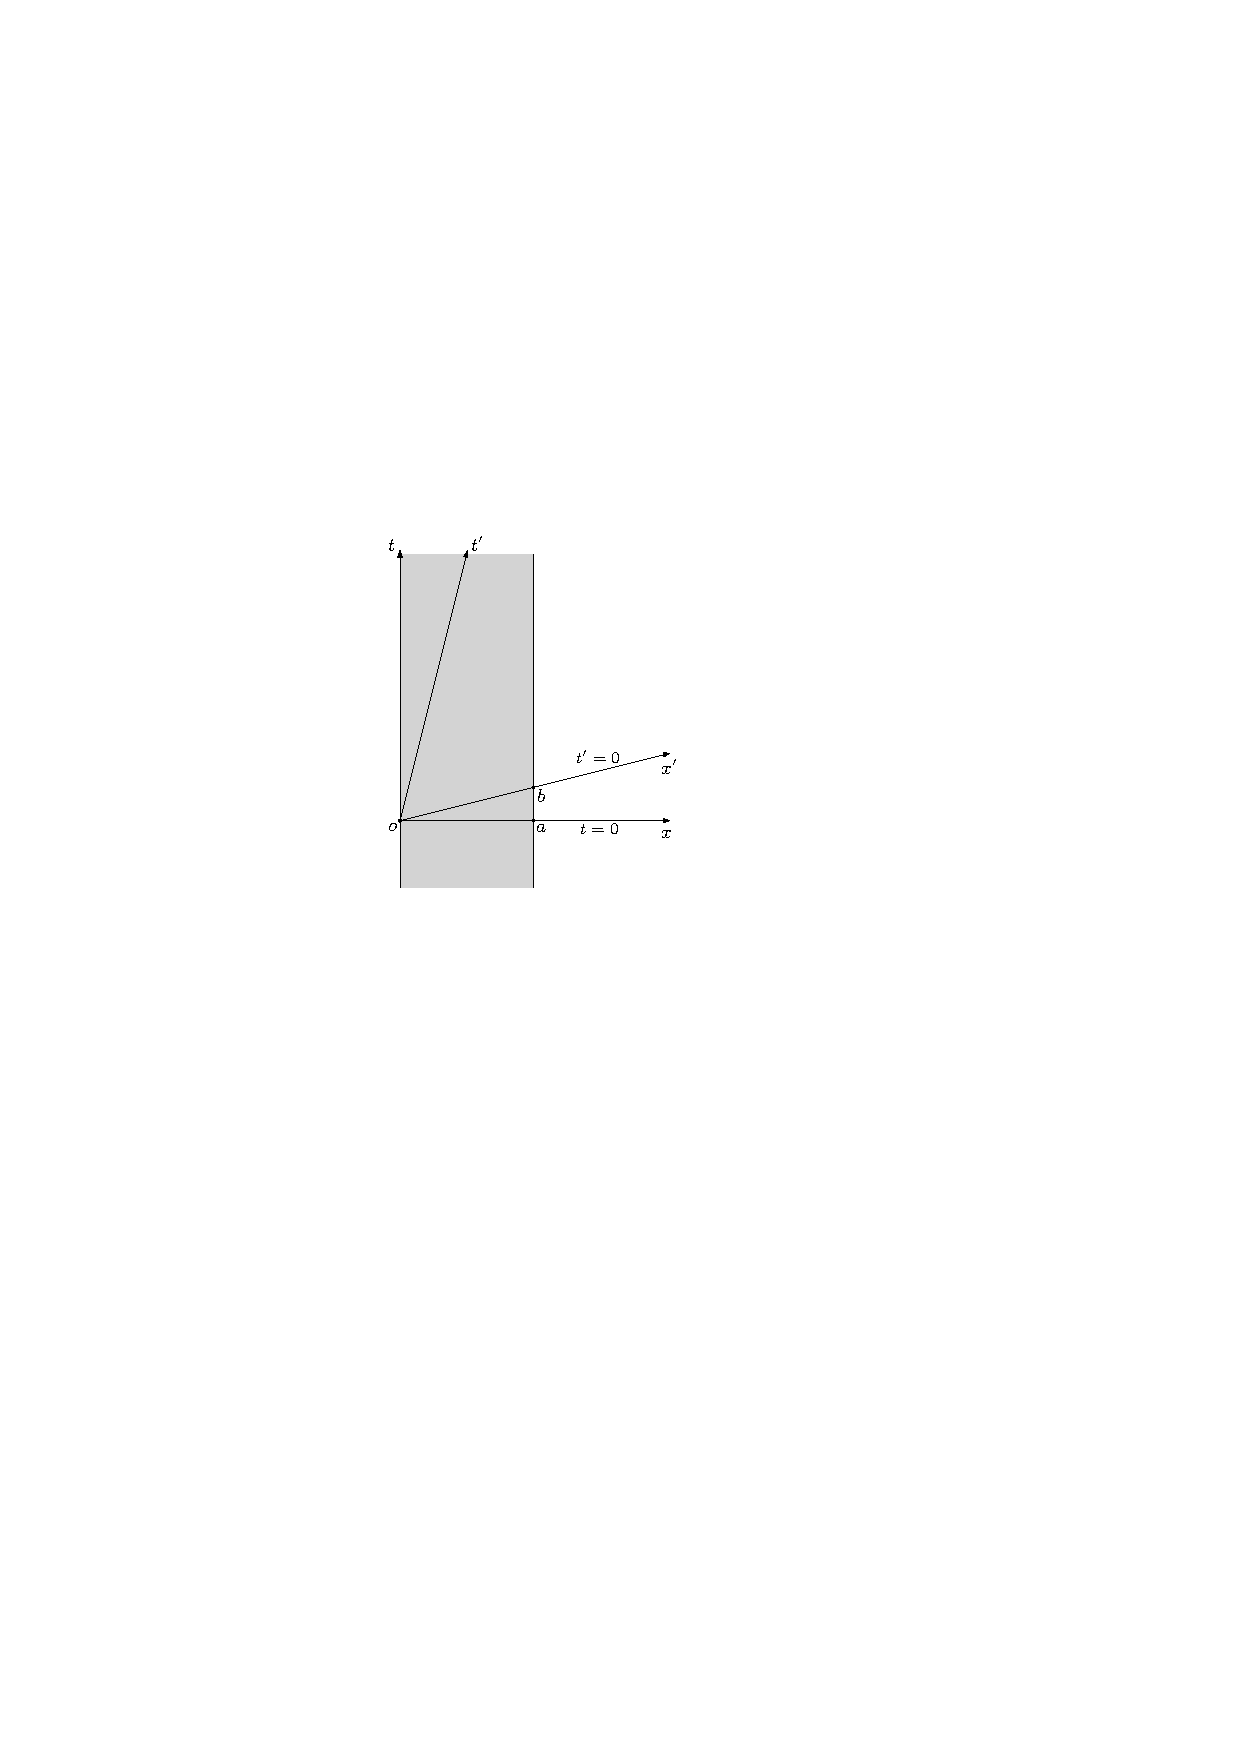
\includegraphics[width=0.4\textwidth]{pic/length contraction.pdf}
    \caption{length contraction}
    \label{length contraction}
\end{figure}

\subsection{双生子佯谬}
如图 \ref{twin paradox} 所示, $ A $ 和 $ B $ 分别以不同的路线从 $ p $ 走到 $ q $, 惯性观者 $ A $ 所经历的时间要小于非惯性观者 $ B $ 所经历的时间.

\begin{figure}[H]
    \centering
    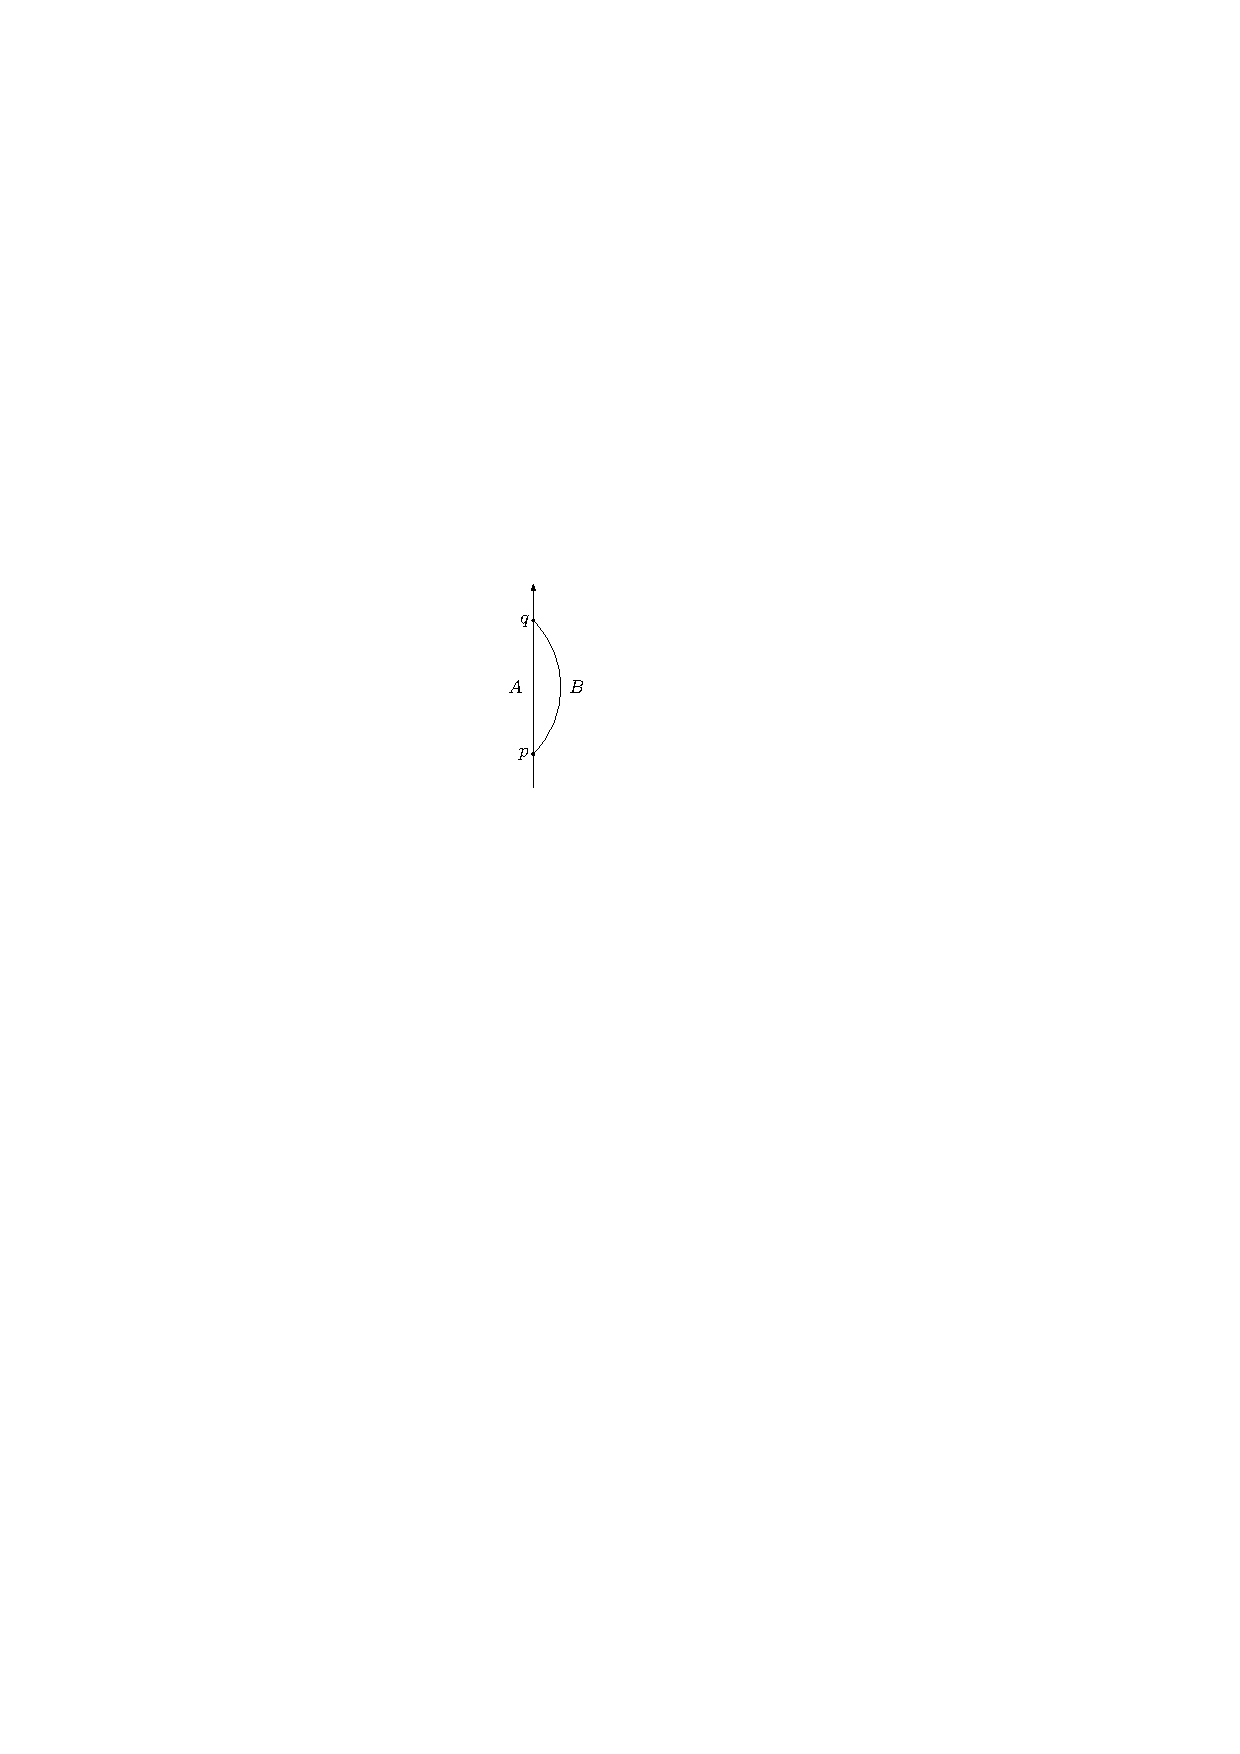
\includegraphics[width=0.2\textwidth]{pic/twin paradox.pdf}
    \caption{twin paradox}
    \label{twin paradox}
\end{figure}
